
\section{Troubleshooting}

	\subsection{Installation}

	\begin{itemize}
	\item Compilation fails, with an error due to send calls for MPI.  

	You are probably using OpenMPI, and their implementation does not use {\tt const}-correctness.  Daniel needs to modify the code in {\tt bertini_extensions} to cast away constness for these send calls.  Send him an email to poke him.  Or, use a different implementation of MPI.  MPICH2, versions 3.04 and up are known to compile using the code as written. 
	\end{itemize}

\subsection{Bertini}

\subsection{Bertini\_real}


\subsubsection{\tt had a critical failure}

\paragraph{Missing critical points, or curve slicing problems}

Sometimes when decomposing an object, Bertini\_real will display something like

{\tt	had a critical failure
 moving left was deficient 2 points
trying to recover the failure...
tracktolBEFOREeg: 1e-07 tracktolDURINGeg: 1e-08
}

This is generally due to a missing critical point.  Bertini\_real uses linear product regeneration to compute critical points, and a missing critical point will cause errors as above.  

The solution to this problem is to get Bertini to not miss any critical points.  This means understanding the path tracker, and what settings influence tracking success.  I generally find several settings can positively influence computation of critical points:
\begin{itemize}
\item {\tt securitymaxnorm}, {\tt securitylevel}

 This is the norm of path truncation during the endgame, during path tracking in Bertini.  If two successive approximations of points on a path exceed this norm, the path will be truncated, unless {\tt securitylevel} is set to {\tt 1}.  Setting the security level to 1 will make tracking take longer, as all paths which end at $\infty$ are tracked all the way to the end.  So level 0 spares computation.  However, during computation of critical points, synthetic variables representing nullspaces of Jacobians are used, and these can have large norms, resulting in truncation of paths which we need to succeed to fully decompose the object.  

Hence, we recommend setting securitymaxnorm to something large but not crazy large.  This is naturally problem dependent.  Somewhere around 1e14 has proven useful in our experiments.  YMMV.

To prevent any paths from being truncated, use {\tt securitylevel 1}.

\item {\tt condnumthreshold}

The post-processor in Bertini classifies endpoints of paths as singular on several criteria, including multiplicity, and on condition number of the Jacobian.  To prevent classification of endpoints as singular, raise this threshold.  Sometimes large values are needed, upwards of perhaps 1e30 or beyond.  

\item {\tt sharpendigits}

After tracking, for nonsingular endpoints Newton's method can be run to increase the accuracy of approximations.  This setting sets the number of digits you wish for.  You are not guaranteed this number, because numerical conditioning may prevent sharpening from completing.

\end{itemize}









\subsection{Matlab}

\subsubsection{\tt sh: matlab: command not found}

If you get the message {\tt sh: matlab: command not found} from running Bertini\_real, then Matlab is not on your shell path.  Bertini\_real currently requires Matlab to run properly, and thus failure to include the Matlab executable on the path will cause bertini\_real to fail. Below is an example of the terminal output displayed when Bertini\_real is unable to locate the Matlab executable: 
 
\begin{center}\begin{minipage}{0.9\linewidth}
\centering
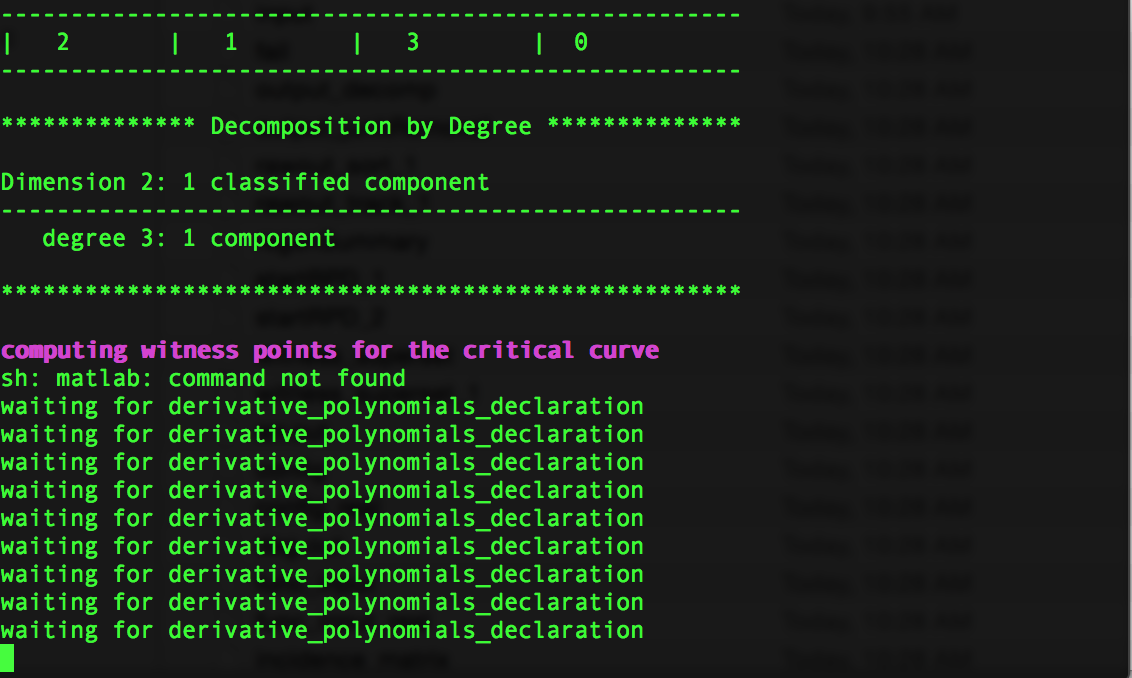
\includegraphics[width=0.6\textwidth]{MATLABExecutableFailure}
\end{minipage}\end{center}

Permanently fixing this error involves editing your profile, e.g. \texttt{bash\_profile}. From your home directory, open \texttt{.bash\_profile} and add the following line: \texttt{export \gls{path}=/PATH/TO/MATLAB.app/bin:\$PATH} where \texttt{PATH/TO/MATLAB.app} points to the location of the Matlab executable. If you do not have, type \texttt{touch .bash\_profile}, which will create \texttt{.bash\_profile}, and then add \texttt{export \gls{path}=/PATH/TO/MATLAB.app/bin:\$PATH}. This should result in the Matlab executable being added to the path whenever opening terminal. 




\subsubsection{Calling Bertini\_real from within Matlab}

Note that you cannot run Bertini\_real from within Matlab, even with the use of {\tt !}, because Bertini\_real currently calls Matlab using a {\tt system()} call. 


\subsubsection{Removing dependency on Matlab's symbolic toolbox}



Removal of Matlab as a dependency is ongoing work.  Please consider helping me move to Python or another open source language for the symbolic computations, required for deflation of singular curves, and the writing of the input file for critical curves of surfaces.
